\documentclass[10pt]{beamer}

\usepackage{color}
\usepackage{listings}

\usetheme{Hannover}
\usefonttheme{serif}
\usecolortheme{seagull}
\beamertemplatenavigationsymbolsempty
\setbeamertemplate{blocks}[rounded][shadow=false]
\setbeamertemplate{bibliography item}{\insertbiblabel}

\definecolor{Blue}{rgb}{0.0, 0.0, 0.8}
\definecolor{DarkGreen}{rgb}{0.0, 0.5, 0.0}
\definecolor{DarkGray}{rgb}{0.5, 0.5, 0.5}
\definecolor{Gray}{rgb}{0.8, 0.8, 0.8}
\definecolor{Orange}{rgb}{0.8, 0.5, 0.0}
\definecolor{White}{rgb}{1.0, 1.0, 1.0}

\lstset{
  basicstyle=\ttfamily\footnotesize,
  breakatwhitespace=false,
  breaklines=true,
  captionpos=b,
  commentstyle=\color{DarkGreen},
  escapeinside={\%*}{*)},
  extendedchars=true,
  frameshape={RYR}{Y}{Y}{RYR},
  keepspaces=true,
  keywordstyle=\color{Blue},
  numbers=left,
  numbersep=6pt,
  numberstyle=\tiny\color{DarkGray},
  rulecolor=\color{Gray},
  showspaces=false,
  showstringspaces=false,
  showtabs=false,
  stepnumber=1,
  stringstyle=\color{Orange},
  tabsize=2
}

\title{X86 Operating System From Scratch}
\subtitle{
  How Hard Can It Be?
  \vspace{0.5cm}
  \\
  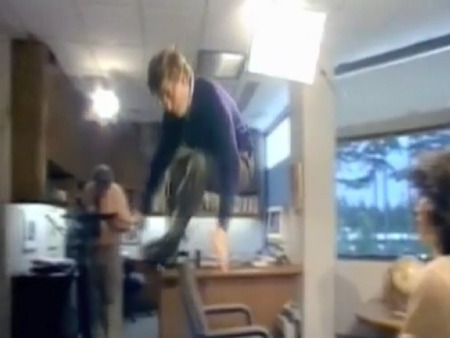
\includegraphics[height=3cm,keepaspectratio]{chair-jump.jpg}
  \\
  \scriptsize{\emph{Bill Gates jumping an office chair}}
}
\author[UH CSS]{D.~Barry\inst{1}}
\institute{
  \inst{1}
  Computer Science Society
  \\
  University of Hertforshire
}
\date{January, 2017}
\subject{Computer Science}

\begin{document}
  %%%%%%%%%%%%%%%%%%%%%%%%%%%%%%%%%%%%%
  % Title
  %%%%%%%%%%%%%%%%%%%%%%%%%%%%%%%%%%%%%
  \frame{\titlepage}
  \begin{frame}
    \frametitle{Table of Contents}
    \begin{block}{}
      \vspace{0.5cm}
      \tableofcontents
      \vspace{0.5cm}
    \end{block}
  \end{frame}
  %%%%%%%%%%%%%%%%%%%%%%%%%%%%%%%%%%%%%
  % Introduction
  %%%%%%%%%%%%%%%%%%%%%%%%%%%%%%%%%%%%%
  \section[Intro]{Introduction}
  \begin{frame}
    \frametitle{What Is An OS?}
    Let us define it by what we expect from it:
    \begin{itemize}
      \item Boots the computer and prepares it for a program to run.
      \item Provides a level of abstraction from the low level hardware (e.g.
        memory management, disk operations, etc).
      \item Allows programs to use predetermined functions, allowing for easier
        writing of programs.
    \end{itemize}
    \centering{
      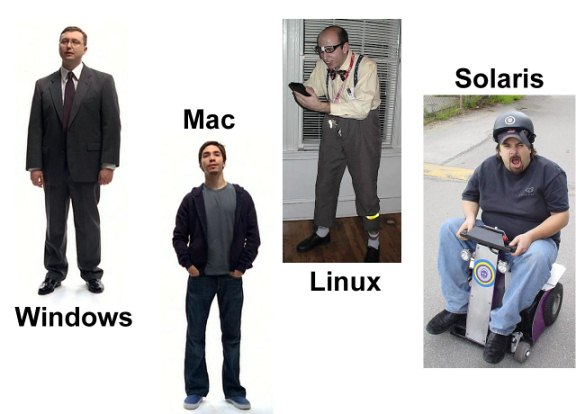
\includegraphics[height=4cm,keepaspectratio]{os-compare.jpg}
      \cite{oscomp}
    }
  \end{frame}
  \begin{frame}
    \frametitle{Why Build An OS?}
    \begin{itemize}
      \item General curiosity
      \item Advancing knowledge
      \item Fun project
      \item I always wanted my own [My Name] OS
      \item I want to be [Bill Gates/Steve Jobs/Linus Torvalds]
    \end{itemize}
    \centering{
      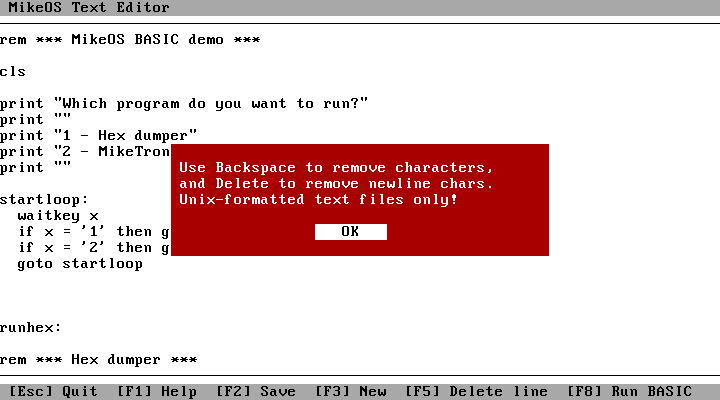
\includegraphics[height=4cm,keepaspectratio]{mikeos-editor.png}
      \cite{mikeos}
    }
  \end{frame}
  \begin{frame}
    \frametitle{What OS Will We Build?}
    \begin{itemize}
      \item 16 bit
      \item 16kB RAM
      \item Custom File System
      \item Command Line
      \item Monolithic
    \end{itemize}
    \centering{
      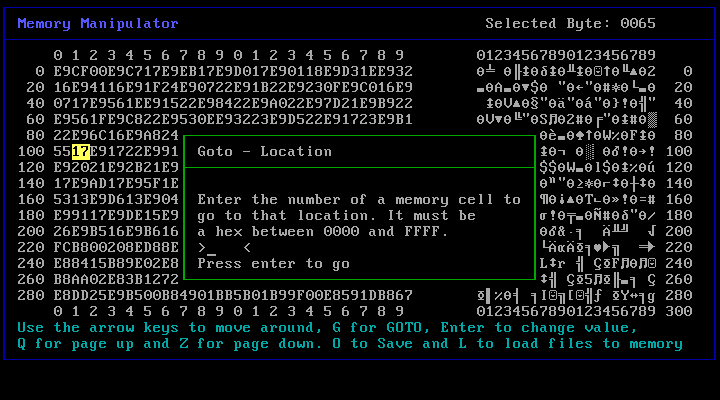
\includegraphics[height=4cm,keepaspectratio]{mikeos-memory.png}
      \cite{mikeos}
    }
  \end{frame}
  %%%%%%%%%%%%%%%%%%%%%%%%%%%%%%%%%%%%%
  % Development Environment
  %%%%%%%%%%%%%%%%%%%%%%%%%%%%%%%%%%%%%
  \section[Dev]{Development}
  \begin{frame}
    \frametitle{Resources}
    You will need:
    \begin{itemize}
      \item Some virtualiation software (\url{https://www.virtualbox.org/} or
        \url{http://www.vmware.com/})
      \item Image Creator (can be downloaded)
      \item NASM (can be downloaded)
    \end{itemize}
    You can download the core resources from
    \url{http://coffeespace.org.uk/downloads/os-from-scratch.zip}.
    \centering{
      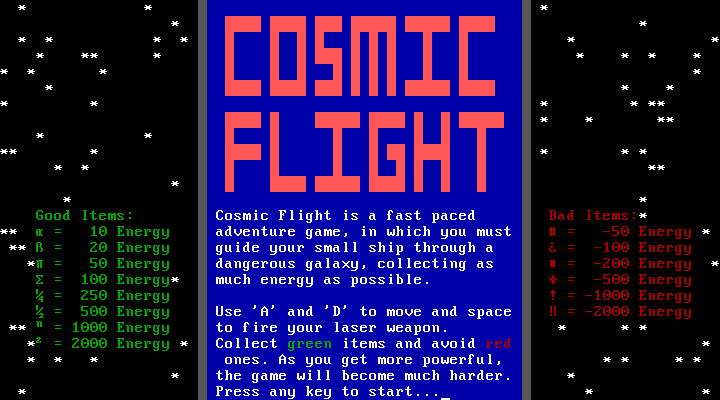
\includegraphics[height=4cm,keepaspectratio]{mikeos-flight.png}
      \cite{mikeos}
    }
  \end{frame}
  \begin{frame}
    \frametitle{Image Creator}
    \begin{itemize}
      \item Allows the custom creation of disk images
      \item Command line utility, use: \texttt{./ic.jar -h} for information
      \item Custom software written in Java
    \end{itemize}
    \centering{
      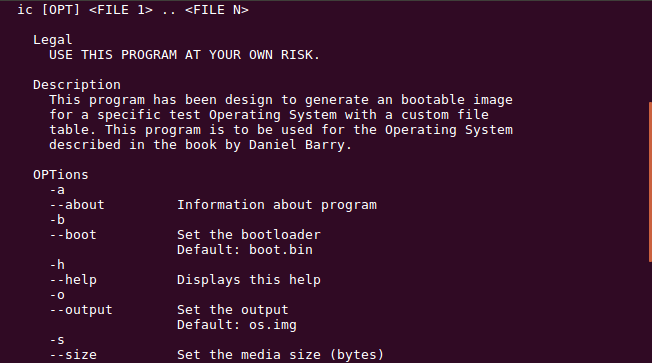
\includegraphics[height=4cm,keepaspectratio]{image-creator.png}
    }
  \end{frame}
  \begin{frame}
    \frametitle{NASM}
    \begin{itemize}
      \item Compiler for assmebly code to machine code
      \item Well tested, well documented
      \item Other compilers will unlikely work
    \end{itemize}
    \centering{
      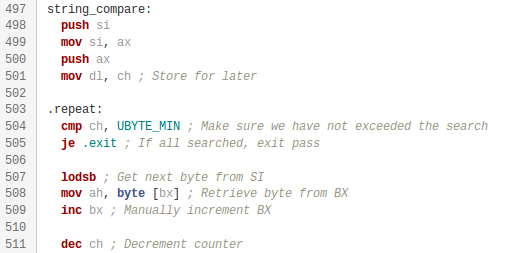
\includegraphics[height=4cm,keepaspectratio]{nasm-code.png}
      \cite{nasmus}
    }
  \end{frame}
  %%%%%%%%%%%%%%%%%%%%%%%%%%%%%%%%%%%%%
  % Coding
  %%%%%%%%%%%%%%%%%%%%%%%%%%%%%%%%%%%%%
  \section[Code]{Coding}
  \begin{frame}
    \frametitle{Getting Started}
    \begin{itemize}
      \item A good starting point is on page 5 of the book in the download,
        under the heading ``Build Environment".
      \item Advanced users can skip to page 8, under the heading ``Bootloader".
    \end{itemize}
  \end{frame}
  %%%%%%%%%%%%%%%%%%%%%%%%%%%%%%%%%%%%%
  % Introduction
  %%%%%%%%%%%%%%%%%%%%%%%%%%%%%%%%%%%%%
  \section[Reff]{References}
  \begin{frame}
    \frametitle{References}
    \begin{thebibliography}{}
      \bibitem{oscomp}
        PinStake,
        ``Windows Vs Mac Vs Linux",
        \emph{PinStake.com},
        \url{http://pinstake.com/windows-vs-mac-vs-linux-windows-mac-linux},
        2017.
      \bibitem{mikeos}
        Saunders, M.
        ``X86 Operating System",
        \emph{SourceForget.net},
        \url{http://mikeos.sourceforge.net/},
        2017.
      \bibitem{nasmus}
        Anvin, H.,
        Kukunas, K.,
        Gorcunov, C.,
        Kotler, F.
        ``NASM",
        \emph{nasm.us},
        \url{http://www.nasm.us/},
        2017.
    \end{thebibliography}
  \end{frame}
\end{document}
